Dans ce chapitre, nous décrivons la mise en œuvre des analyses statiques
précédentes. Nous commençons par un tour d'horizon des représentations
intermédiaires possibles, avant de décrire celle retenue : Newspeak. La chaîne
de compilation est explicitée, partant de C pour aller au langage impératif
décrit dans le chapitre~\ref{cha:lang}. Enfin, nous donnons les détails d'un
algorithme d'inférence de types à la Hindley-Milner, reposant sur l'unification
et le partage de références.

%\begin{tabular}{| l || l | l | l | l | l | l |}
\hline
Nom           & Langage hôte    & Description       & But                 & Langage source                   &  Sémantique & Types \\ \hline \hline
C             & Texte           & \cite{AnsiC}      & Compilation         & C                                &  Non        & Oui   \\ \hline
GIMPLE        & C               & \cite{gcc-gimple} & Compilation         & C + extensions, C++, Ada, \ldots &  Non        & Non   \\ \hline
LLVM          & C++             & \cite{llvm-pres}  & Compilation         & C + extensions, C++, Ada, \ldots &             & Oui   \\ \hline
Cminusminus   & Texte           & \cite{spjcmm}     & Compilation         &                                  &             & Oui   \\ \hline
Cmm (Haskell) & Texte / Haskell &                   & Compilation         &                                  &             &       \\ \hline
Cmm (OCaml)   & OCaml           &                   & Compilation         &                                  &             &       \\ \hline
CIL           & OCaml           & \cite{NeculaCil}  & Analyse             &                                  &             &       \\ \hline
Clight        & Coq             & \cite{cfront}     & Compilation/Analyse &                                  &  Oui        & Oui   \\ \hline
Cminor        & Coq             & \cite{cminorSL}   & Compilation/Analyse &                                  &  Oui        & Oui   \\ \hline
Newspeak      & Ocaml           & \cite{newspeak}   & Analyse             &                                  &  Oui        & Oui   \\ \hline
\end{tabular}

% vim: textwidth=0


\section{Newspeak}
\label{sec:npk}

Newspeak~\cite{newspeak} est un langage conçu pour être à la fois :

\begin{itemize}
  \item \textbf{Précis} : sa sémantique est définie formellement
  \cite{HymansLevillainEADS08}
  \item \textbf{Expressif} : la plupart des primitives présentes dans les
    langages de bas niveau sont compilables en Newspeak \footnote{Penjili étant
    spécialisé dans l'aéronautique, les constructions complexes comme
    \texttt{longjmp} / \texttt{setjmp} ou les exceptions ne sont pas nécessaires.}
    % TODO adapter la footnote
  \item \textbf{Simple} : peu de primitives sont présentes.
  \item \textbf{Minimal} : aucun élément syntaxique ne peut être exprimé
    comme combinaison d'autres.
  \item \textbf{Explicite} : les constructions sont toutes indépendantes du
    contexte.
  \item \textbf{Orienté analyse} : les primitives sont décorées d'informations
    reflétant leur validité (tests de bornes, etc)
  \item \textbf{Indépendant de l'architecture} : toutes les caractéristiques comme
    la taille des types ou l'alignement des structures sont rendues explicites.
\end{itemize}

\section{Chaîne de compilation}

\begin{figure}
  \centering
  \begin{tikzpicture}\shorthandoff{!}
\tikzstyle{file}=[draw, shape=rectangle, node distance=2.2cm, minimum
height=1cm, shade, top color=white,
    bottom color=blue!50!black!20, draw=blue!40!black!60, very thick];

\node [file] (c1) {\textcolor{black}{.c}};
\node [file, below of=c1] (c2) {\textcolor{black}{.c}};
\node [node distance=2.2cm, below of=c2] (c3) {};

\node [file, minimum height=0, node distance=5mm, above of=c3,draw] (c3b) {.adb};
\node [file, minimum height=0, node distance=5mm, below of=c3,draw] (c3s) {.ads};

\path (c3b.north west) ++(-3mm,3mm) [draw,dotted] rectangle ($(c3s.south east)+(3mm,-3mm)$);

\node [below of=c3, node distance=2.2cm] (c4){};

\node [file, right of=c1] (cc1) {\textcolor{black}{.c}};
\node [file, right of=c2] (cc2) {\textcolor{black}{.c}};
\node [node distance=2.2cm, right of=c3] (cc3) {};

\node [below of=cc3, node distance=2.2cm](cc4){};

\draw[->] (c1) -- node[above] {{\tiny \ttfamily cpp}} (cc1);
\draw[->] (c2) -- (cc2);

\node [file, right of=cc1] (no1) {\textcolor{black}{.no}};
\node [file, right of=cc2] (no2) {\textcolor{black}{.no}};
\node [file, right of=cc3] (no3) {\textcolor{black}{.no}};

\node [below of=no3, node distance=2.2cm](no4){};

\draw[->] (cc1) -- node[above] {{\tiny \ttfamily c2newspeak -c}} (no1);
\draw[->] (cc2) --  (no2);

\draw[->] ($ (c3b.north east)!0.5!(c3s.south east) + (3mm,0) $) -- node[above] {\tiny \ttfamily ada2newspeak -c} (no3);


\node [file, right of=no2] (npk) {\textcolor{black}{.npk}};

\node [right of=no3, node distance=2.2cm](npk2){};
\node [right of=no4, node distance=2.2cm](npk3){};

\node[draw, ellipse, right of=no2, minimum height=3cm]{};

\draw[->] (no1) -- node {} (npk);
\draw[->] (no2) -- node[above] {{\tiny \ttfamily c2newspeak}} (npk);
\draw[->] (no3) -- node {} (npk);


\node [file, right of=npk, node distance=3cm, yshift=1cm](warn)
    {\textcolor{black}{\parbox{2cm}{\centering Programme \linebreak typé}}};
\node [right of=npk, node distance=3cm, yshift=-1cm](warnn)
    {\textcolor{black}{Erreurs}};

\node [right of=npk3, node distance=3cm](analyser2){};

\node [right of=npk, node distance=3cm] {\small ou};

\draw[->] (npk) -- node[above, yshift=2mm] {{\tiny \ttfamily ptrtype}} (warn);

\draw[->] (npk) -- (warnn);

\draw[->] (c4)   -- node[above, text depth=3pt] {\footnotesize Pr\'etraitement} (cc4);
\draw[->] (cc4)  -- node[above, text depth=3pt] {\footnotesize Compilation} (no4);
\draw[->] (no4)  -- node[above, text depth=3pt] {\footnotesize \'Edition de liens} (npk3);
\draw[->] (npk3) -- node[above, text depth=3pt] {\footnotesize Analyse} (analyser2);
\end{tikzpicture}

  \caption{Compilation depuis Newspeak}
  \label{fig:compil-npk}
\end{figure}

%TODO Mettre à jour la figure

La compilation vers C est faite en trois étapes (figure~\ref{fig:compil-npk}) :
prétraitement du code source, compilation de C prétraité vers \newspeak{}, puis
compilation de \newspeak{} vers ce langage.

\section*{Trad}

La première étape consiste à prétraiter les fichiers C source avec le logiciel
\texttt{cpp}, comme pour une compilation normale. Cette étape interprète les
directives comme \texttt{\#include}, \texttt{\#ifdef}, À cet étape, les
commentaires sont aussi supprimés.

% TODO comment interpréter les /*!npk xxx */ ?

Pour que le code noyau soit compilable, il est nécessaire de définir certaines
macros. En particulier, le système de configuration de Linux utilise des macros
nommées \texttt{CONFIG\_*} pour inclure ou non certaines fonctionnalités. Il a
donc fallu faire un choix ; nous avons choisi la configuration par défaut. Pour
analyser des morceaux plus importants du noyau, il faudrait définir un fichier
de configuration plus important.

% TODO ce para peut aller dans le chapitre cas d'étude

Une fois cette passe effectuée, nous avons des fichiers C prétraités,
c'est à dire des unités de compilation autocontenues. % TODO bof

Puisque la directive \texttt{\#include} est textuelle, ces fichiers sont très
grands et donnent lieu à beaucoup de duplication dans les passes suivantes.

À ce niveau, les fichiers sont passés à l'outil \texttt{c2newspeak} qui les
traduit vers Newspeak. Dans cette étape, les types et les noms sont résolus, et
le programme est annoté de manière à rendre les prochaines étapes indépendante
du contexte. Par exemple, chaque déclaration de variable est adjointe d'une
description complète du type.

Puisque Linux est écrit dans le dialecte ``GNU C'', il a été nécessaire
d'adapter \texttt{c2newspeak}. La principale particularité est la notation
\texttt{\_\_attribute\_\_((...))} qui peut décorer les déclarations de
fonctions, de variables ou de types. De nouvelles fonctionnalités sont aussi
présentes.

Par exemple, il est possible de manipuler des étiquettes de première classe : si
\texttt{lbl:} est présent avant une instruction, on peut capturer l'adresse de
celle-ci avec \texttt{void *p = \&\&lbl} et y sauter indirectement avec
\texttt{goto *p}.

Une autre fonctionnalité est le concept d'instruction-expression :
\texttt{(\{bloc\})}) est une expression, dont la valeur est celle de la dernière
expression évaluée lors de \texttt{i}.

Les attributs, quant à eux, rentrent dans trois catégories :

\begin{itemize}
  \item les annotations de compilation ; par exemple, \texttt{used} désactive
    l'avertissement ``cette variable n'est pas utilisée ''.

  \item les optimisations ; par exemple, les objets marqués \texttt{hot} sont
    groupés de telle manière qu'ils se retrouvent en cache ensemble.

  \item les annotations de bas niveau ; par exemple, \texttt{aligned(n)}
    spécifie qu'un objet doit être aligné sur au moins \texttt{n} bits.
\end{itemize}

Dans notre cas, toutes ces annotations peuvent être ignorées.

% TODO pê tout ça dans le chap suivant

Lors de cette étape, le flôt de contrôle est également simplifié. C en effet
propose de nombreuses constructions ambigües ou redondantes.

Au contraire, Newspeak propose un nombre réduit de constructions. Rappelons que
le but de ce langage est de faciliter l'analyse statique : des constructions
orthogonales permettent donc d'éviter la duplication de règles sémantique, ou de
code lors de l'implémentation d'un analyseur.

Par exemple, plutôt que de fournir une boucle \emph{while}, une boucle
\emph{do/while} et une boucle for, Newspeak fournit une unique boucle
\npkWhile{}. La sortie de boucle est compilée vers un \npkGoto{}\cite{goto}, qui est
toujours un saut vers l'avant (similaire à un "break" généralisé).

La sémantique de Newspeak et la traduction de C vers Newspeak sont décrites dans
\cite{newspeak}.

Newspeak est conçu pour l'analyse statique par interprétation abstraite. Il a
donc une vue de bas niveau sur les programmes. Par exemple, aucune distinction
n'est faite entre l'accès à un champ et l'accès un l'élément d'un tableau (tous
deux sont traduits par un décalage numérique depuis le début de la zone
mémoire). Pour supprimer cette ambiguïté, il faut s'interfacer dans les
structures internes de \texttt{c2newspeak}, où les informations nécessaires sont
encore présentes.

Ensuite, les différents fichiers sont liés ensemble. Cet étape consiste
principalement à s'assurer que les hypothèses faites par les différentes unités
de compilation sont cohérentes entre elles. Les objets marqués \texttt{static},
invisibles à l'extérieur de leur unité de compilation, sont renommés afin qu'ils
aient un nom unique.

Enfin, l'implantation d'un algorithme d'inférence pour les systèmes de types
décrits dans les chapitres~\ref{cha:typbase} et~\ref{cha:qualifs} est assez
simple. Puisqu'ils sont suffisament proches du lambda calcul simplement typé, on
peut utiliser une variante de l'algorithme W de Damas et
Milner~\cite{DamasMilner}. On utilise l'optimisation classique qui consiste à se
reposer sur le partage de références pour réaliser l'unification, plutôt que de
faire des substitutions explicites. Puisque ces systèmes de types sont
monomorphes, on présente une erreur si des variable de type libres sont
présentes.

À la fin de cette étape, on obtient soit un programme complètement annoté, soit
une erreur de type.

\subsection{Prétraitement}

\ctonewspeak{} travaillant uniquement sur du code prétraité (dans directives de
préprocesseur), la première étape consiste donc à faire passer le code par \cpp:
les macros sont développées, les constantes remplacées par leurs valeurs, les
commentaires supprimés, les fichiers d'en-tête inclus, etc.

\subsection{Compilation (levée des ambigüités)}

Cette passe est réalisée par l'utilitaire \ctonewspeak{}. L'essentiel de la
compilation consiste à mettre à plat les définition de types, et \subsection{Annotations}

\newspeak{} a de nombreux avantages, mais pour une analyse par typage il est
trop bas niveau. Par exemple, dans le code suivant

\begin{Verbatim}[commandchars=\\\{\}]
\PY{k}{struct} \PY{n}{s} \PY{p}{\PYZob{}}
    \PY{k+kt}{int} \PY{n}{a}\PY{p}{;}
    \PY{k+kt}{int} \PY{n}{b}\PY{p}{;}
\PY{p}{\PYZcb{}}\PY{p}{;}

\PY{k+kt}{int} \PY{n+nf}{main}\PY{p}{(}\PY{k+kt}{void}\PY{p}{)}
\PY{p}{\PYZob{}}
    \PY{k}{struct} \PY{n}{s} \PY{n}{x}\PY{p}{;}
    \PY{k+kt}{int} \PY{n}{y}\PY{p}{[}\PY{l+m+mi}{10}\PY{p}{]}\PY{p}{;}
    \PY{n}{x}\PY{p}{.}\PY{n}{b} \PY{o}{=} \PY{l+m+mi}{1}\PY{p}{;}
    \PY{n}{y}\PY{p}{[}\PY{l+m+mi}{1}\PY{p}{]} \PY{o}{=} \PY{l+m+mi}{1}\PY{p}{;}
    \PY{k}{return} \PY{l+m+mi}{0}\PY{p}{;}
\PY{p}{\PYZcb{}}
\end{Verbatim}


\wip{}

\subsection{Implantation de l'algorithme de typage}

On prend l'exemple d'un lambda-calcul simplement typé avec entiers, flottants et
couples (figure~\ref{fig:stlc}).

\begin{figure}

\gramlr{Termes}{
\begin{align*}
  t \gramisa & x              & \textrm{Variable} \\
    \gramor  & λ x . t        & \textrm{Abstraction} \\
    \gramor  & t              & \textrm{Application} \\
    \gramor  & n              & \textrm{Entier} \\
    \gramor  & f              & \textrm{Flottant} \\
    \gramor  & (t, t)         & \textrm{Couple} \\
    \gramor  & \textrm{fst}~t & \textrm{Projection gauche} \\
    \gramor  & \textrm{snd}~t & \textrm{Projection droite}
\end{align*}
}

\gramlr{Types}{
\begin{align*}
  τ \gramisa &  \tInt          & \textrm{Entier}\\
    \gramor  &  \tFloat        & \textrm{Flottant}\\
    \gramor  & τ \rightarrow τ & \textrm{Fonction} \\
    \gramor  & τ \times τ      & \textrm{Produit}
\end{align*}
}

\gramlr{Contextes}{
\begin{align*}
  Γ \gramisa & ε     & \textrm{Contexte vide}\\
    \gramor  & Γ,x:τ & \textrm{Extension}
\end{align*}
}

\gramlr{Règles}{
\begin{mathpar}
\irule{Int}{ }{Γ⊢n:\tInt}
\and
\irule{Float}{ }{Γ⊢f:\tFloat}
\and
\irule{Var}{x:τ∈Γ}{Γ⊢x:τ}
\and
\irule{App}{Γ⊢f:τ_1 \rightarrow τ_2 \\ Γ ⊢ x : τ_1}{Γ ⊢ f x : τ_2}
\and
\irule{Abs}{Γ,x:τ_1⊢ y : τ_2}{Γ⊢ λx.y:τ_1 \rightarrow τ_2}
\and
\irule{Proj-g}{Γ⊢x:τ_1\times τ_2}{Γ⊢\textrm{fst}~x:τ_1}
\and
\irule{Proj-d}{Γ⊢x:τ_1\times τ_2}{Γ⊢\textrm{snd}~x:τ_2}
\and
\irule{Tup}{Γ⊢x:τ_1 \\ Γ⊢y:τ_2}{Γ⊢(x,y):τ_1 \times τ_2}
\end{mathpar}
}


\caption{Lambda calcul simplement typé avec entiers, flottants et couples}
\label{fig:stlc}

\end{figure}

Prenons l'exemple de la fonction suivante\footnote{ On suppose que \texttt{plus}
est une fonction de l'environnement global qui a pour type $\tInt \rightarrow
\tInt \rightarrow \tInt$.} :

\[
f = λx.λy. \textrm{plus} (\textrm{plus} (\textrm{fst} x) (\textrm{snd} x)) y
\]

Soit en syntaxe ML :

\begin{Verbatim}
let f x y =
  plus
    (plus
      (fst x)
      (snd x)
    )
    y
\end{Verbatim}

Puisque \texttt{fst} et \texttt{snd} sont appliqués à \texttt{x}, ce doit être
un tuple. En outre on additionne ces deux composantes ensemble, donc elles
doivent être de type \tInt (et le résultat aussi). Par le même argument,
\texttt{y} doit aussi être de type \tInt. En conclusion, \texttt{x} est de type
$\tInt × \tInt$ et \texttt{y} de type $\tInt$, donc f est de type $\tInt × \tInt
→ \tInt → \tInt$.

Pour implanter cette analyse, on peut remarquer qu'étant donné la forme d'un
terme, on peut savoir quelle règle de typage a été utilisée en dernier. Il est
ainsi possible de ``remonter'' l'arbre d'inférence afin de savoir quelles règles
ont été employées (figure~\ref{fig:inftree-rules})\footnote{Par souci de clarté,
les prémisses des applications de \textsc{(Var)} ne sont pas notées.}. Pour le
moment, on ne connait pas les types.

% TODO quel prop cela utilise t'il?

\begin{figure} % {{{ Fig règles
\def\disptypeR#1#2{:#1}

\def\gammaXY{\ensuremath{Γ_2}}
\def\gammaX{\ensuremath{Γ_1}}
\def\gammaOneDef{\ensuremath{Γ^0, x\disptypeL{\tInt \times \tInt}, y\disptypeL{\tInt}}}
\def\gammaTwoDef{\ensuremath{Γ^0, x\disptypeL{\tInt \times \tInt}}}
\def\termFst#1{\ensuremath{\textrm{fst}~x}}
\def\termSnd#1{\ensuremath{\textrm{snd}~x}}
\def\fstx{\termFst{x}}
\def\sndx{\termSnd{x}}
\begin{mathpar}
\irule
  {Abs}
  {
    \irule
      {Abs}
      {
        \inferrule*[right=(App)]
          {
            \inferrule*[right=(Var), rightskip=4em]
              { }
              {\gammaXY ⊢ y
              \disptypeR{\tInt}
              }
            \\
            \inferrule*[right=(App),vdots=4em,leftskip=5em,rightskip=5em]
              {
                \inferrule*[right=(Var), leftskip=3em, rightskip=7em]
                  { }
                  {\gammaXY ⊢ \textrm{plus}
                  \disptypeR{\tInt \rightarrow \tInt \rightarrow \tInt}
                  }
                \\
                \inferrule*[right=(App),vdots=3em,leftskip=7em,rightskip=3em]
                  {
                    \inferrule*[right=(App), vdots=4em, rightskip=5em]
                      {
                        \inferrule*[right=(Var), rightskip=5em]
                          { }
                          {\gammaXY ⊢ \textrm{plus}
                          \disptypeR{\tInt \rightarrow \tInt \rightarrow \tInt}
                          }
                        \\
                        \inferrule*[right=(Proj-G), vdots=3em, leftskip=5em]
                          {
                            \irule
                              {Var}
                              { }
                              {\gammaXY ⊢ x
                              \disptypeR{\tInt \times \tInt}
                              }
                          }
                          {\gammaXY ⊢ \fstx
                          \disptypeR{\tInt}
                          }
                      }
                      {\gammaXY ⊢ \textrm{plus} (\fstx)
                      \disptypeR{\tInt \rightarrow \tInt}
                      }
                    \\
                    \inferrule*[right=(Proj-D), leftskip=5em, rightskip=4em]
                      {
                        \irule
                          {Var}
                          { }
                          {\gammaXY ⊢ x
                          \disptypeR{\tInt \times \tInt}
                          }
                      }
                      {\gammaXY ⊢ \sndx
                      \disptypeR{\tInt}
                      }
                  }
                  {\gammaXY ⊢ \textrm{plus} (\fstx) (\sndx)
                  \disptypeR{\tInt}
                  }
              }
              {\gammaXY ⊢ \textrm{plus} (\textrm{plus} (\fstx) (\sndx))
              \disptypeR{\tInt \rightarrow \tInt}
              }
          }
          {\gammaXY ⊢ \textrm{plus} (\textrm{plus} (\fstx) (\sndx)) y
          \disptypeR{\tInt}
          }
      }
      {\gammaX ⊢ λy. \textrm{plus} (\textrm{plus} (\fstx) (\sndx)) y
      \disptypeR{\tInt \rightarrow \tInt}
      }
  }
  {Γ_0 ⊢ λx.λy. \textrm{plus} (\textrm{plus} (\fstx) (\sndx)) y
  \disptypeR{\tInt \times \tInt \rightarrow \tInt \rightarrow \tInt}
  }
\end{mathpar}

\[\gammaX = \gammaTwoDef \qquad \gammaXY = \gammaOneDef\]


\caption{Arbre d'inférence : règles à utiliser}
\label{fig:inftree-rules}
\end{figure} % }}}

Une fois à cette étape, on peut donner un nom à chaque type inconnu : $t_1, t_2,
\ldots$. L'utilisation qui en est faite permet de générer un ensemble de
contraintes d'unification. Par exemple, pour chaque application de la règle
\textsc{(App)} de la forme :

\[
\irule{App}{Γ⊢\ldots:t_3 \\ Γ ⊢ \ldots : t_1}{Γ ⊢ \ldots : t_2}
\]

on doit déduire que $t_3 = t_1 \rightarrow t_2$.

\begin{figure}
\centering

\subbottom[Contraintes]{
  \label{fig:inf-constr-ex}
  \begin{minipage}{0.5\linewidth}
  \begin{align}
  t_1    &= t_x → t_2             \tag{Abs1} \\
  t_2    &= t_y → t_3             \tag{Abs2} \\
  t_5    &= t_4 → t_3             \tag{App1} \\
  t_4    &= t_y                   \tag{Var1} \\
  t_6    &= t_7 → t_5             \tag{App2} \\
  t_6    &= \tInt → \tInt → \tInt \tag{Var2} \\
  t_{10} &= t_8 → t_7             \tag{App3} \\
  t_9    &= ? × t_8               \tag{Proj-D1} \\
  t_9    &= t_x                   \tag{Var3} \\
  t_{11} &= t_{12} → t_{10}       \tag{App4} \\
  t_{11} &= \tInt → \tInt → \tInt \tag{Var4} \\
  t_{13} &= t_{12} × ?            \tag{Proj-G1} \\
  t_{13} &= t_x                   \tag{Var5}
  \end{align}
  \end{minipage}
}
\subbottom[Solution]{
  \label{fig:inf-sol-ex}
  \begin{minipage}{0.3\linewidth}
  \begin{align*}
  t_{1}  &= \tInt × \tInt → \tInt \\
  t_{2}  &= \tInt → \tInt         \\
  t_{3}  &= \tInt                 \\
  t_{4}  &= \tInt                 \\
  t_{5}  &= \tInt → \tInt         \\
  t_{6}  &= \tInt → \tInt → \tInt \\
  t_{7}  &= \tInt                 \\
  t_{8}  &= \tInt                 \\
  t_{9}  &= \tInt × \tInt         \\
  t_{10} &= \tInt → \tInt         \\
  t_{11} &= \tInt → \tInt → \tInt \\
  t_{12} &= \tInt                 \\
  t_{13} &= \tInt × \tInt         \\
  t_{x}  &= \tInt × \tInt         \\
  t_{y}  &= \tInt
  \end{align*}
  \end{minipage}
}

\caption{Contraintes d'égalité et solution obtenues à partir de la
figure~\ref{fig:inftree-rules}}

\end{figure}

% TODO mal numéroté

On en déduit donc un ensemble de contraintes d'égalité
(figure~\ref{fig:inf-constr-ex}). D'après (App1) et (App2), $t_6 = t_7 → t_4 →
t_3$ d'où par (Var2), $t_7 → t_4 → t_3 = \tInt → \tInt → \tInt$. Le constructeur
$→$ étant injectif, on a donc $t_3 = t_4 = t_7 = \tInt$. En procédant de même
avec (App3) et (App4), on obtient $t_8 = t_{12} = \tInt$. D'après (Proj-G1),
(Var5), (Var3), et (Proj-D1) on a $t_{12} × ? = t_{13} = t_{x} = t_9 = ? ×
t_{8}$, donc $t_x = t_{12} × t_8 = \tInt × \tInt$. En remplaçant, on obtient
tous les autres types (figure~\ref{fig:inf-sol-ex}).


\clearpage

Ce signe $=$ est à prendre comme une contrainte d'égalité : partant d'un
ensemble de contraintes de la forme "type avec inconnue = type avec inconnue",
on veut obtenir une substitution "inconnue -> type concret".

Pour résoudre ces contraintes, on commence par les simplifier : si $t_a
\rightarrow t_b = t_c \rightarrow t_d$, alors $t_a = t_c$ et $t_b = t_d$. De
même si $t_a \times t_b = t_c \times t_d$. Au contraire, si $t_a \rightarrow t_b
= t_c \times t_d$, il est impossible d'unifier les types et il faut abandonner
l'inférence de types. D'autre cas sont impossibles, par exemple $\tInt = t_1
\rightarrow t_2$ ou $\tInt = \tFloat$.

\begin{figure} % {{{ Fig full tree
\def\disptypeR#1#2{:#2}

\def\gammaXY{\ensuremath{Γ_2}}
\def\gammaX{\ensuremath{Γ_1}}
\def\gammaOneDef{\ensuremath{Γ^0, x\disptypeL{\tInt \times \tInt}, y\disptypeL{\tInt}}}
\def\gammaTwoDef{\ensuremath{Γ^0, x\disptypeL{\tInt \times \tInt}}}
\def\termFst#1{\ensuremath{\textrm{fst}~x}}
\def\termSnd#1{\ensuremath{\textrm{snd}~x}}
\def\fstx{\termFst{x}}
\def\sndx{\termSnd{x}}
\begin{mathpar}
\irule
  {Abs}
  {
    \irule
      {Abs}
      {
        \inferrule*[right=(App)]
          {
            \inferrule*[right=(Var), rightskip=4em]
              { }
              {\gammaXY ⊢ y
              \disptypeR{\tInt}
              }
            \\
            \inferrule*[right=(App),vdots=4em,leftskip=5em,rightskip=5em]
              {
                \inferrule*[right=(Var), leftskip=3em, rightskip=7em]
                  { }
                  {\gammaXY ⊢ \textrm{plus}
                  \disptypeR{\tInt \rightarrow \tInt \rightarrow \tInt}
                  }
                \\
                \inferrule*[right=(App),vdots=3em,leftskip=7em,rightskip=3em]
                  {
                    \inferrule*[right=(App), vdots=4em, rightskip=5em]
                      {
                        \inferrule*[right=(Var), rightskip=5em]
                          { }
                          {\gammaXY ⊢ \textrm{plus}
                          \disptypeR{\tInt \rightarrow \tInt \rightarrow \tInt}
                          }
                        \\
                        \inferrule*[right=(Proj-G), vdots=3em, leftskip=5em]
                          {
                            \irule
                              {Var}
                              { }
                              {\gammaXY ⊢ x
                              \disptypeR{\tInt \times \tInt}
                              }
                          }
                          {\gammaXY ⊢ \fstx
                          \disptypeR{\tInt}
                          }
                      }
                      {\gammaXY ⊢ \textrm{plus} (\fstx)
                      \disptypeR{\tInt \rightarrow \tInt}
                      }
                    \\
                    \inferrule*[right=(Proj-D), leftskip=5em, rightskip=4em]
                      {
                        \irule
                          {Var}
                          { }
                          {\gammaXY ⊢ x
                          \disptypeR{\tInt \times \tInt}
                          }
                      }
                      {\gammaXY ⊢ \sndx
                      \disptypeR{\tInt}
                      }
                  }
                  {\gammaXY ⊢ \textrm{plus} (\fstx) (\sndx)
                  \disptypeR{\tInt}
                  }
              }
              {\gammaXY ⊢ \textrm{plus} (\textrm{plus} (\fstx) (\sndx))
              \disptypeR{\tInt \rightarrow \tInt}
              }
          }
          {\gammaXY ⊢ \textrm{plus} (\textrm{plus} (\fstx) (\sndx)) y
          \disptypeR{\tInt}
          }
      }
      {\gammaX ⊢ λy. \textrm{plus} (\textrm{plus} (\fstx) (\sndx)) y
      \disptypeR{\tInt \rightarrow \tInt}
      }
  }
  {Γ_0 ⊢ λx.λy. \textrm{plus} (\textrm{plus} (\fstx) (\sndx)) y
  \disptypeR{\tInt \times \tInt \rightarrow \tInt \rightarrow \tInt}
  }
\end{mathpar}

\[\gammaX = \gammaTwoDef \qquad \gammaXY = \gammaOneDef\]


\caption{Arbre d'inférence complet}
\label{fig:inftree-full}
\end{figure} % }}}

Une fois ces simplifications réalisées, les contraintes restantes sont d'une des
formes suivantes :

\begin{itemize}
\item
  $t_i = t_i$. Il n'y a rien à faire, cette contrainte peut être supprimée.
\item
  $t_i = t_j$ avec $i \ne j$ : toutes les occurrences de $t_j$ dans les autres
  contraintes peuvent être remplacées par $t_i$.
\item
  $t_i = x$ (ou $x = t_i$) où $x$ est un type concret : idem.
\end{itemize}

%TODO C'est faux

Une fois toutes les substitutions effectuées, on obtient un arbre de typage
correct (figure~\ref{fig:inftree-full}, donc un programme totalement inféré.

\clearpage

\begin{figure} % fig:unifpartage {{{

  \subbottom{
  \label{fig:unifpartage:a}
  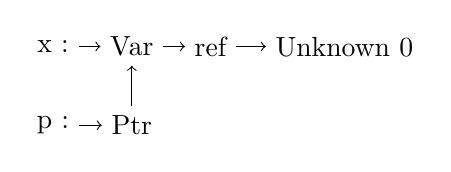
\begin{tikzpicture}
  \node               (var) {Var};
  \node[right of=var] (ref) {ref};
  \node[right of=ref, node distance=1.7cm] (u0) {Unknown 0};
  \node[below of=var] (ptr) {Ptr};
  \node[left of=var]  (x) {x :};
  \node[left of=ptr] (p) {p :};
  \draw[->] (x) -- (var);
  \draw[->] (p) -- (ptr);
  \draw[->] (ptr) -- (var);
  \draw[->] (var) -- (ref);
  \draw[->] (ref) -- (u0);
  \end{tikzpicture}
  }
  \subbottom{
  \label{fig:unifpartage:b}
  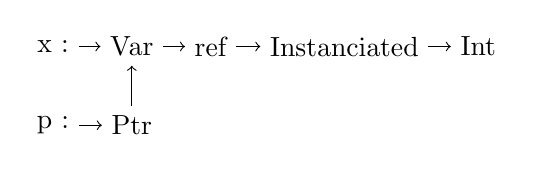
\begin{tikzpicture}
  \node               (var) {Var};
  \node[right of=var] (ref) {ref};
  \node[right of=ref, node distance=1.7cm] (u0) {Instanciated};
  \node[right of=u0, node distance=1.7cm] (ii) {Int};
  \node[below of=var] (ptr) {Ptr};
  \node[left of=var]  (x) {x :};
  \node[left of=ptr] (p) {p :};
  \draw[->] (x) -- (var);
  \draw[->] (p) -- (ptr);
  \draw[->] (ptr) -- (var);
  \draw[->] (var) -- (ref);
  \draw[->] (ref) -- (u0);
  \draw[->] (u0) -- (ii);
  \end{tikzpicture}
  }
  \subbottom{
  \label{fig:unifpartage:c}
  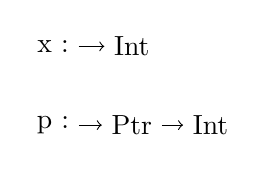
\begin{tikzpicture}
  \node               (var) {Int};
  \node[below of=var] (ptr) {Ptr};
  \node[left of=var]  (x) {x :};
  \node[left of=ptr] (p) {p :};
  \node[right of=ptr] (pi) {Int};
  \draw[->] (x) -- (var);
  \draw[->] (p) -- (ptr);
  \draw[->] (ptr) -- (pi);
  \end{tikzpicture}
  }

  \caption{Unification par partage}
  \label{fig:unifpartage}

\end{figure} % }}}

Plutôt que de modifier toutes les occurrences d'un type $t_i$, on va affecter à
$t_i$ la valeur du nouveau type.

L'implémentation de cet algorithme utilise le partage et les références
(figure~\ref{fig:unifpartage}).

D'abord \ref{fig:unifpartage:a}, ensuite \ref{fig:unifpartage:b}, et enfin
\ref{fig:unifpartage:c}.

\begin{figure} % fig:exunif:c {{{

  \insertcode{ex-unif-c.c}

  \caption{Compilation d'un programme C - avant}
  \label{fig:exunif:c}
\end{figure} % }}}

Prenons l'exemple de la figure~\ref{fig:exunif:c} et typons-le "à la main". On
commence par oublier toutes les étiquettes de type présentes dans le programme.
Celui-ci devient alors :

\insertcode{exunif-code.c}

La premiere ligne introduit deux variables. On peut noter leurs types respectifs
(inconnus pour le moment) $t_1$ et $t_2$. La première affectation \texttt{p =
\&x} implique que les deux côtés du signe "=" ont le même type. À gauche, le
type est $t_2$, et à droite $Ptr(t_1)$. On applique le même raisonnement à la
seconde affectation : à gauche, le type est $t_1$ et à droite Int. On en déduit
que le type de x est Int et celui de p est Ptr(Int).


\insertcode{lambda-types.ml}

Pour implanter cet algorithme, on représente les types de données du programmes
à typer par une valeur de type \texttt{ml\_type}. En plus des constantes de
types comme int ou float, et des constructeurs de type comme pair et fun, le
constructeur Var permet d'exprimer les variables de types (inconnues ou non).

Celles-ci sont numérotées par un int, on suppose avoir à disposition deux
fonctions manipulant un compteur global d'inconnues.

\insertcode{exunif-counter.ml}

De plus, on a un module gérant les environnements de typage. Il pourra être
implanté avec des listes d'association ou des tables de hachage, par exemple. Sa
signature est :

\insertcode{exunif-env.ml}

Reprenons l'exemple précédent. Partant d'un environnement vide (Env.empty), on
commence par l'étendre de deux variables. Comme on n'a aucune information, il
fait allouer des nouveaux noms d'inconnues (qui correspondent à $t_1$ et $t_2$):

\insertcode{exunif-1.ml}

La première instruction indique que les deux côtés de l'affectation doivent
avoir le même type.

\insertcode{exunif-2.ml}

\begin{figure}
  \centering
  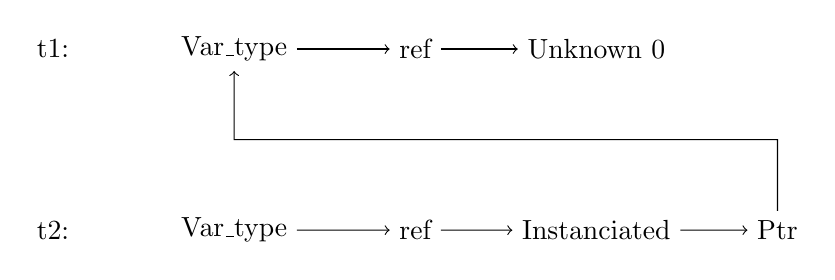
\begin{tikzpicture}
    [scale=2.3]

    \node at (0,  0) (n0a) {t1:};
    \node at (0, -1) (n0b) {t2:};

    \node at (1,  0) (n1a) {Var\_type};
    \node at (2,  0) (n2a) {ref};
    \node at (3,  0) (n3a) {Unknown 0};

    \node at (1, -1) (n1b) {Var\_type};
    \node at (2, -1) (n2b) {ref};
    \node at (3, -1) (n3b) {Instanciated};
    \node at (4, -1) (n4b) {Ptr};

    \draw [->] (n1a) -- (n2a);
    \draw [->] (n2a) -- (n3a);

    \draw [->] (n1b) -- (n2b);
    \draw [->] (n2b) -- (n3b);
    \draw [->] (n3b) -- (n4b);

    \draw [->] (n4b) -- ++ (0, 0.5) -| (n1a);

  \end{tikzpicture}
  \caption{Unification : partage}
  \label{fig:unifsharing}
\end{figure}

Ici il se passe plusieurs choses intéréssantes. D'une part nous faisont appel à
une fonction externe typeof qui retourne le type d'une expression sous un
environnement (dans une implantation complète il s'agirait d'un appel récursif).
Dans ce cas, \texttt{typeof lhs1 env} est identique à \texttt{Env.get lhs1 env}
et \texttt{typeof rhs1 env} à \texttt{Ptr\_type t1}. L'autre aspect intéressant
est la dernière ligne : la fonction \texttt{unify} va modifier en place les
représentations des types afin de les rendre égales. L'implantation de
\texttt{unify} sera décrite plus tard. Dans ce cas précis, elle va faire pointer
la référence dans t2 vers t1 (figure~\ref{fig:unifsharing}).

Enfin, la seconde affectation se déroule à peu près de la même manière.

\insertcode{exunif-3.ml}

Ici \texttt{typeof lhs2 env} est identique à \texttt{Ptr\_type (Env.get "p"
env)} et \texttt{typeof lhs2 env} à \texttt{Const\_type Int\_type}. Et dans cas,
l'unification doit se faire entre t1 et \texttt{Const\_type Int\_type} : cela
mute la référence derrière t1 (figure~\ref{fig:typeunifref}).

\begin{figure}
  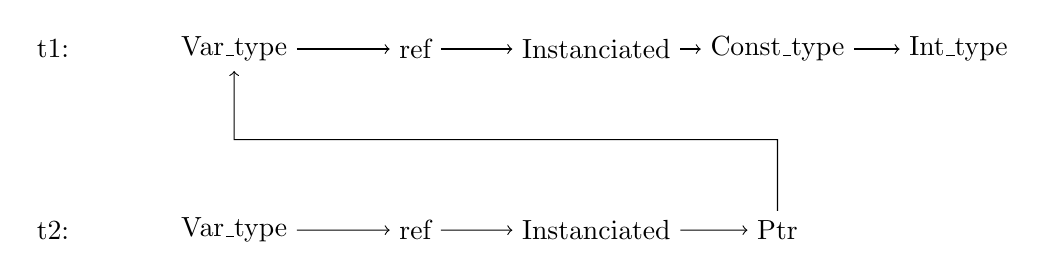
\begin{tikzpicture}
    [scale=2.3]

    \node at (0,  0) (n0a) {t1:};
    \node at (0, -1) (n0b) {t2:};

    \node at (1,  0) (n1a) {Var\_type};
    \node at (2,  0) (n2a) {ref};
    \node at (3,  0) (n3a) {Instanciated};
    \node at (4,  0) (n4a) {Const\_type};
    \node at (5,  0) (n5a) {Int\_type};

    \node at (1, -1) (n1b) {Var\_type};
    \node at (2, -1) (n2b) {ref};
    \node at (3, -1) (n3b) {Instanciated};
    \node at (4, -1) (n4b) {Ptr};

    \draw [->] (n1a) -- (n2a);
    \draw [->] (n2a) -- (n3a);
    \draw [->] (n3a) -- (n4a);
    \draw [->] (n4a) -- (n5a);

    \draw [->] (n1b) -- (n2b);
    \draw [->] (n2b) -- (n3b);
    \draw [->] (n3b) -- (n4b);

    \draw [->] (n4b) -- ++ (0, 0.5) -| (n1a);

  \end{tikzpicture}
  \caption{Unification par mutation de références}
  \label{fig:typeunifref}
\end{figure}

L'essence de l'algorithme d'inférence se situe donc dans 2 fonctions. D'une
part, \texttt{unify} qui réalise l'unification des types grâce à au partage des
références. D'autre part, la \texttt{typeof} qui encode les règles de typage
elles-mêmes et les applique à l'aide de \texttt{unify}.

\subsection{Algorithme d'unification}

Voici une implantation de la fonction \texttt{unify}.

Celle-ci prend en entrée deux types $t_1$ et $t_2$. À l'issue de l'exécution de
\texttt{unify}, ces deux types doivent pouvoir être considérés comme égaux. Si
ce n'est pas possible, une erreur sera levée.

La première étape est de réduire ces deux types, c'est à dire à transformer les
constructions \texttt{Var (ref (Instanciated t))} en \texttt{t}.

Ensuite, cela dépend des formes qu'ont les types réduits :

\begin{figure}
  \centering
  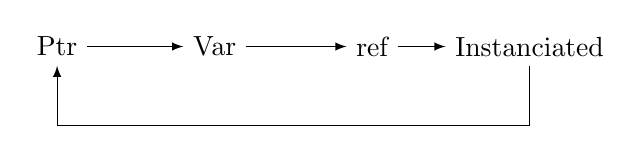
\begin{tikzpicture}
    [every node/.style={node distance=2cm}
    ,>=latex
    ]

    \node (n1) {Ptr};
    \node[right of=n1] (n2) {Var};
    \node[right of=n2] (n3) {ref};
    \node[right of=n3] (n4) {Instanciated};

    \draw [->] (n1) -- (n2);
    \draw [->] (n2) -- (n3);
    \draw [->] (n3) -- (n4);

    \draw [->] (n4) -- ++ (0, -1cm) -| (n1);

  \end{tikzpicture}
  \caption{Cycle dans le graphe de types}
  \label{fig:typecycle}
\end{figure}

\begin{itemize}

\item si les deux types sont inconnus (de la forme \texttt{Var (ref
(Instanciated t))}), on fait pointer l'une des deux références vers le premier
type. Notons que cela crée un type de la forme \texttt{Var (ref (Instanciated
(Var (ref (Unknown n)))))} qui sera réduit lors d'une prochaine étape
d'unification.

\item si un type est inconnu et pas l'autre, il faut de la même manière affecter la
référence. Mais en faisant ça inconditionnellement, cela peut poser problème :
par exemple en tentant d'unifier \texttt{a} avec \texttt{Ptr(a)} on pourrait
créer un cycle dans le graphe (figure~\ref{fig:typecycle}).
Pour éviter cette situation, il suffit de s'assurer que le type inconnu n'est
pas présent dans le type à affecter.

\item si les deux types sont des types de base (comme \tInt ou \tFloat) égaux,
on ne fait rien.

\item si les deux types sont des constructeurs de type, il faut que les
constructeurs soient égaux. On unifie en outre leurs arguments deux à deux.

\item dans les autres cas, l'algorithme échoue.

\item TODO sous typage pour les structures

\end{itemize}


TODO :

\begin{itemize}
\item implem du polymorphisme
\item implem du sous-typage
\item généralisation depuis le toy language
\end{itemize}

\clearpage

\begin{figure} % fig:exunif:tpk {{{

  \insertcode{ex-unif-tpk.ml}

  \caption{Compilation d'un programme C - après}
  \label{fig:exunif:tpk}
\end{figure} % }}}

Le programme C (figure~\ref{fig:exunif:c}) est compilé ainsi en Tyspeak
(figure~\ref{fig:exunif:tpk}).

\section*{Extrait PLAS}

The language described above, as well as a type inference algorithm, have been
implemented in OCaml as part of the Newspeak framework of program
analysis\cite{newspeak}. It is released under the GNU Lesser General Public
License, and is available on \texttt{http://penjili.org} (directory
\texttt{src/ptrtype} in the distribution). Our implementation consists of the
following steps.

but to analyze larger parts of the kernel, it may be
necessary to define a ``maximal'' configuration file (which is impossible
because of incompatibilities between some options).



Let us run the analysis on a small example:

\begin{verbatim}
int f(int *x) { return (*x + 1); }
\end{verbatim}

Running our analyzer outputs a fully annotated program:

\begin{verbatim}
 % ptrtype example.c
f : (Ptr (Int)) -> (Int)
Int (example.c:1#4)^f(Ptr (Int) x) {
  (.c:3#4)^!return =(int32)
    (coerce[-2147483648,2147483647]
      ( ( ([(x_Ptr (Int) : Ptr (Int))]32_Int
            : Int
          )
          + (1 : Int)
        ) : Int
      ) : Int
    );
}
\end{verbatim}

The \texttt{coerce[a,b]} operator is a Newspeak artifact to detect integer
overflows when doing a value analysis by abstract interpretation. For the
purposes of this paper, it can be seen as the identity function typed
$(\tInt) → \tInt$.

\emph{A contrario}, when it is not possible to type check, the analyzer bails
out with an error.

\begin{verbatim}
void f(int *p) {
    /*!npk userptr p */
    *p = 3;
}
\end{verbatim}

The \texttt{/*!npk userptr p */} comment is interpreted by the analyzer and
causes it to unify the type of \texttt{p} with $t~\qUser~*$, effectively
forcing its qualifier.

\begin{verbatim}
04-addrof.c:4#4 - Cannot unify qualifiers:
  Kernel
  User
\end{verbatim}

We just signal the location where a unification failed, but it is possible to
keep track of all the unification sites to create a trace, easier to debug.



% vim: spelllang=fr
